\chapter{Modelação Lógica}

% tirar isto? ou é melhor deixar e tentar incorporar?
%\section{Construção e validação do modelo de dados lógico}

Nesta capítulo, traduzimos o modelo concetual (fig. \ref{fig:concetual}) num modelo de dados lógico adequado aos dados do ginásio. Para tal, seguimos o processo descrito em \cite{dbsys}.

\section{Derivar relações para o modelo de dados lógicos}

Começamos por derivar relações a partir do modelo concetual seguindo as regras adequadas, de modo a representar no modelo lógico as entidades, relacionamentos e atributos identificados previamente. Tal gerou as seguintes relações. No entanto, para as relações Cliente e Funcionário, decidimos separar os atributos compostos \emph{Contacto} e \emph{Morada} nas suas próprias relações, em vez de colocar os respetivos atributos atómicos nas relações mencionadas, de forma a facilitar a compreensão.


\noindent
\\\textbf{Cliente} (ClienteID,  Nome, DataNascimento, Sexo, Peso, Altura, IMC, Limitações Físicas,  NrContribuinte, idContacto, idMorada)
\\\textbf{Primary Key} ClienteID
\\\textbf{Foreign Key} idContacto \textbf{references} Contacto(idContacto)
\\\textbf{Foreign Key} idMorada \textbf{references} Morada(idMorada)

\noindent
\\\textbf{Contacto} (idContacto, Telemóvel 1, Telemóvel 2, Email)
\\\textbf{Primary Key} idContacto

\noindent
\\\textbf{Morada} (idMorada, Rua, Localidade, CodigoPostal)
\\\textbf{Primary Key} idMorada

\noindent
\\\textbf{Serviço} (ServiçoID, Designação, Preço, Estado)
\\\textbf{Primary Key} ServiçoID

\noindent
\\\textbf{Fatura} (FaturaID, Contribuinte Empresa, Data, Desconto, Descrição, Valor, ClienteID, FuncionárioID, Estado)
\\\textbf{Primary Key} FaturaID
\\\textbf{Foreign Key} ClienteID \textbf{references} Cliente(ClienteID)
\\\textbf{Foreign Key} FuncionárioID \textbf{references} Funcionário(FuncionárioID)

\noindent
\\\textbf{Funcionário} (FuncionárioID, Nome, Cargo, Idade, idContacto, idMorada)
\\\textbf{Primary Key} FuncionárioID
\\\textbf{Foreign Key} idContacto \textbf{references} ContactoFuncionario(idContacto)
\\\textbf{Foreign Key} idMorada \textbf{references} MoradaFuncionario(idMorada)

\noindent
\\\textbf{ContactoFuncionario} (idContacto, Telemóvel 1, Telemóvel 2, Email)
\\\textbf{Primary Key} idContacto

\noindent
\\\textbf{MoradaFuncionario} (idMorada, Rua, Localidade, CodigoPostal)
\\\textbf{Primary Key} idMorada

\noindent
\\\textbf{Exercício} (ExercícioID, Designação, Tipo de Exercício)
\\\textbf{Primary Key} ExercícioID

\noindent
\\\textbf{Equipamento} (EquipamentoID, Descrição, Nome)
\\\textbf{Primary Key} EquipamentoID

% *:* relationship
\noindent
\\\textbf{Constitui} (ServiçoID, FaturaID)
\\\textbf{Primary Key} ServiçoID, FaturaID
\\\textbf{Foreign Key} ServiçoID \textbf{references} Serviço(ServiçoID)
\\\textbf{Foreign Key} FaturaID \textbf{references} Fatura(FaturaID)

% *:* relationship
\noindent
\\\textbf{Subscreve} (ClienteID, ServiçoID, Data Subscrição)
\\\textbf{Primary Key} ClienteID, ServiçoID
\\\textbf{Foreign Key} ClienteID \textbf{references} Cliente(ClienteID)
\\\textbf{Foreign Key} ServiçoID \textbf{references} Serviço(ServiçoID) 

% *:* relationship
\noindent
\\\textbf{E prestado por} (ServiçoID, FuncionárioID, Data Início)
\\\textbf{Primary Key} ServiçoID, FuncionárioID
\\\textbf{Foreign Key} ServiçoID \textbf{references} Serviço(ServiçoID)
\\\textbf{Foreign Key} FuncionárioID \textbf{references} Funcionário(FuncionárioID)

% *:* relationship
\noindent
\\\textbf{Plano Exercícios} (ClienteID, ExercicioID, Numero de Repetições, Numero de Series)
\\\textbf{Primary Key} ClienteID, ExercicioID
\\\textbf{Foreign Key} ClienteID \textbf{references} Cliente(ClienteID)
\\\textbf{Foreign Key} ExercicioID \textbf{references} Exercício(ExercicioID)

% *:* relationship
\noindent
\\\textbf{É utilizado para} (EquipamentoID, ExercícioID)
\\\textbf{Primary Key} EquipamentoID, ExercícioID
\\\textbf{Foreign Key} EquipamentoID \textbf{references} Equipamento(EquipamentoID)
\\\textbf{Foreign Key} ExercícioID \textbf{references} Exercício(ExercícioID)



\section{Desenho do modelo lógico}

A conversão das relações derivadas anteriormente resultou no modelo lógico representado na figura \ref{fig:mod_logico}.

\begin{figure}[h]
\begin{center}
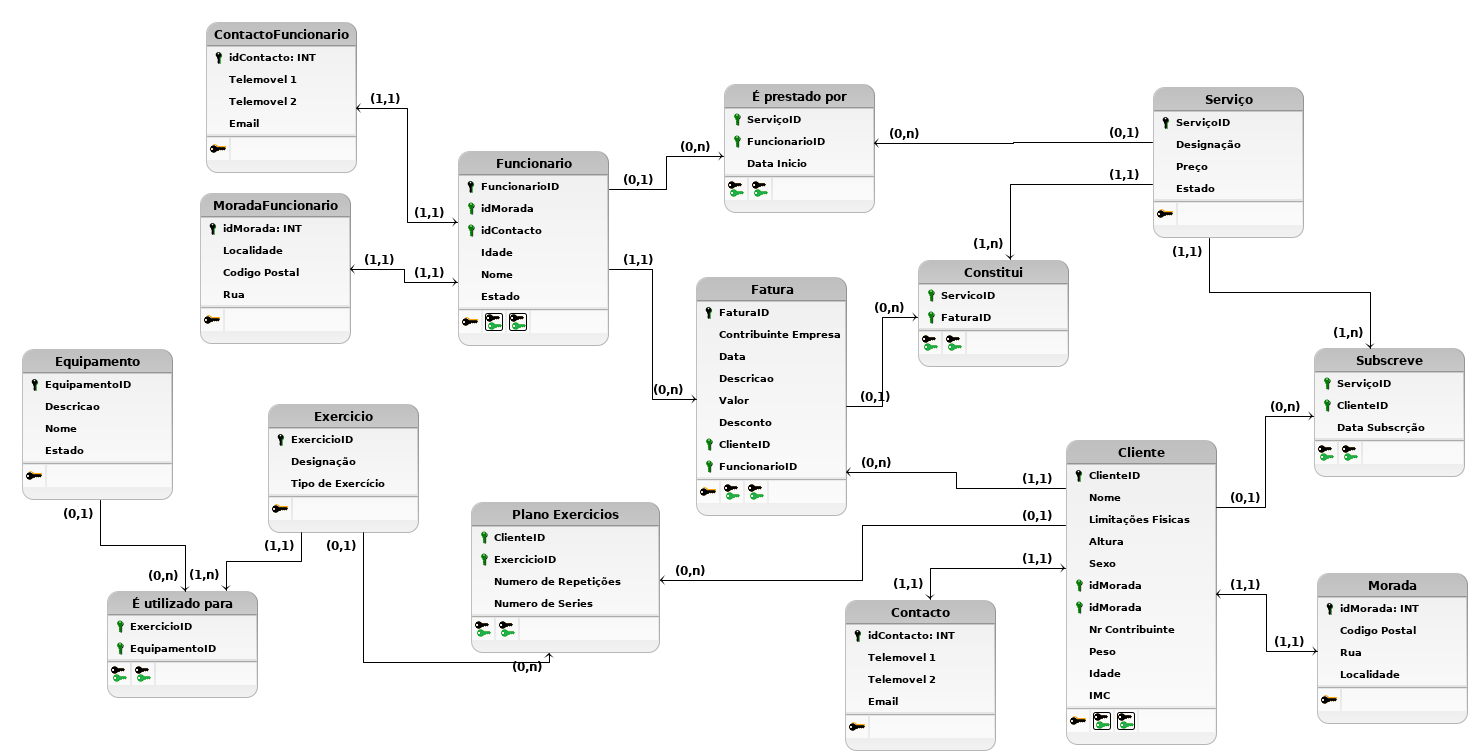
\includegraphics[width=\textwidth]{modelacao_logica/logicoBR.png}
\caption{Modelo Lógico}
\label{fig:mod_logico}
\end{center}
\end{figure}


\section{Validação do modelo através da normalização}

\subsection{Dependências Funcionais}

\noindent
\\\textbf{Cliente:}
\\ClienteID ®  Nome, Idade, Sexo, Peso, Altura, IMC, Limitações Físicas,  NrContribuinte, idContacto, idMorada
\\NrContribuinte ® ClienteID, Nome, Idade, Sexo, Peso, Altura, IMC, Limitações Físicas, idContacto, idMorada
\\idContacto ® ClienteID, Nome, Idade, Sexo, Peso, Altura, IMC, Limitações Físicas, NrContribuinte, idMorada

\noindent
\\\textbf{Contacto:}
\\idContacto ® Telemóvel 1, Telemóvel 2, Email

\noindent
\\\textbf{Morada:}
\\idMorada ® Rua, Localidade, CodigoPostal

\noindent
\\\textbf{Serviço:}
\\ServiçoID ® Designação, Preço

\noindent
\\\textbf{Fatura:}
\\FaturaID ® Contribuinte Empresa, Data, Desconto, Descrição, Valor, ClienteID, FuncionárioID

\noindent
\\\textbf{Funcionário:}
\\FuncionárioID ® Nome, Cargo, Idade, idContacto, idMorada

\noindent
\\\textbf{ContactoFuncionario:}
\\idContacto ® Telemóvel 1, Telemóvel 2, Email

\noindent
\\\textbf{MoradaFuncionario:}
\\idMorada ® Rua, Localidade, CodigoPostal

\noindent
\\\textbf{Exercício:}
\\ExercícioID ® Designação, Tipo de Exercício

\noindent
\\\textbf{Equipamento:}
\\EquipamentoID ® Descrição, Nome

\noindent
\\\textbf{Subscreve:}
\\ClienteID, ServiçoID ® Data Subscrição

\noindent
\\\textbf{E prestado por:}
\\ServiçoID, FuncionárioID ® Data Início

\noindent
\\\textbf{Plano Exercícios:}
\\ClienteID, ExercicioID ® Numero de Repetições, Numero de Series



\subsection{Primeira Forma Normal (1FN)}

Todas as relações estão na Primeira Forma Normal, pois, para cada relação, a interseção de uma linha e uma coluna contém apenas um valor.

\subsection{Segunda Forma Normal (2FN)}

As relações estão na Segunda Forma Normal, pois cada relação está na 1FN e todos os atributos não chave primária dessa relação dependem da totalidade da chave primária.

\subsection{Terceira Forma Normal (3FN)}

As relações estão na Terceira Forma Normal, pois cada relação está na 1FN e na 2FN e todos os atributos não chave primária dessa relação e dependem diretamente da chave primária, ou seja, não existem dependências transitivas.

\section{Validação do modelo com interrogações do utilizador}
\label{interrogacoes}

As seguintes interrogações proveem da secção \ref{subsec:requisitos}, composta por interrogações e transações. Iremos validar estas interrogações verificando que toda a informação necessária à sua realização (entidades, atributos e relacionamentos) está presente no modelo. As transações serão validadas na secção \ref{transacoes}.

\noindent
\\\textbf{Tem de ser possível visualizar que serviços são prestados por que funcionários.}
\\ As entidades Serviço e Funcionário, que compreendem os detalhes dos serviços e dos funcionários, respetivamente, estão representadas no modelo. Podemos usar o relacionamento \emph{Serviço É Prestado Por Funcionário} para extrair a informação requerida.

\noindent
\\\textbf{O responsável do ginásio poderá também consultar os serviços fornecidos pelo ginásio}
\\ $ \pi_{Designacao} (Servico) $

\noindent
\\\textbf{Para posterior confirmação dos updates ou adições referentes ao funcionário, o administrador deverá poder visualizar o conteúdo da tabela dos funcionários}
\\ $ \pi (Funcionario) $

\noindent
\\\textbf{Existe a necessidade de aceder à ficha do cliente pelo número de utilizador}
\\ A entidade Cliente representa os dados do cliente, que tem um número de utilizador único (o atributo ClienteID), logo a operação é possível.

\noindent
\\\textbf{Também deverá ser possível aceder à ficha do cliente através do seu número de telefone, caso este não saiba o seu idCliente}
\\ A entidade Cliente representa os dados do cliente e os contactos dos clientes estão representados na relação Contacto. A entidade Cliente tem como uma \emph{Foreign Key} o identificador do contacto do cliente na tabela Contacto, pelo que é possível associar a um cliente ao seu número de telefone e, assim, aceder aos dados do cliente a partir deste.

\noindent
\\\textbf{Terá de ser possível ao funcionário consultar os exercícios de um cliente}
\\ A entidade Cliente representa os dados do cliente e a entidade Exercício representa os exercícios no modelo lógico. Utilizando o relacionamento \emph{Plano Exercícios}, é possível consultar a informação requerida.

\noindent
\\\textbf{Deverá ser possível a consulta de todas as faturas emitidas pelo ginásio relativas a um cliente}
\\ As entidades Cliente e Fatura representam, respetivamente, os clientes (e os seus dados) e as faturas (e os seus dados). Utilizando o relacionamento \emph{Cliente Tem Fatura}, podemos produzir a lista de todas as faturas relatias a um cliente.

\noindent
\\\textbf{A consulta de faturas entre duas datas específicas será também uma funcionalidade presente na base de dados}
\\ A entidade Fatura, que representa as faturas no modelo lógico, tem um atributo NN \emph{Data}, que guarda a data de emissão da fatura, pelo que a operação é possível.

\noindent
\\\textbf{O responsável reserva-se o dever de ter acesso ao total faturado num determinado período de tempo ou durante todo o tempo de vida do ginásio}
\\ A entidade Fatura, que representa as faturas no modelo lógico, tem um atributo NN \emph{Data}, que guarda a data de emissão da fatura, e um atributo NN \emph{Valor}, que guarda o valor total da fatura, portanto, a interrogação é válida.

\noindent
\\\textbf{Quer o administrador quer os rececionistas devem poder ver que serviços foram registados em cada fatura}
\\ As entidades Serviço e Fatura representam, respetivamente, os serviços providenciados pelo ginásio e as faturas emitidas por este no modelo. Utilizando o relacionamento \emph{Serviço Constitui Fatura}, é possível visualizar a informação pretendida.

\noindent
\\\textbf{Os funcionários devem poder também ver quais as subscrições dos clientes}
\\  As entidades Cliente e Fatura representam, respetivamente, os clientes (e os seus dados) e os serviços do ginásio. Utilizando o relacionamento \emph{Cliente Subscreve Serviço}, é possível saber quais as subscrições dos clientes.


\section{Validação do modelo com as transações estabelecidas}
\label{transacoes}

As seguintes transações proveem da secção \ref{subsec:requisitos}, composta por interrogações e transações. Iremos validar estas transações verificando que toda a informação necessária à sua realização (entidades, atributos e relacionamentos) está presente no modelo. As interrogações foram validadas na secção \ref{interrogacoes}.


\noindent
\\\textbf{Terá de ser possível ao responsável do ginásio adicionar um funcionário}
\\ A entidade Funcionário, que representa os funcionários e os seus dados, existe no modelo, pelo que é possível adicionar funcionários à BD.

\noindent
\\\textbf{Terá também  de ser possível ao administrador do ginásio alterar a informação relativa a um funcionário}
\\ É possível, por consequência direta da existência da entidade Funcionário.

\noindent
\\\textbf{Outra das funções do administrador do ginásio será adicionar novos serviços que poderão vir a ser disponibilizados aos clientes}
\\ A entidade Serviços, que representa os serviços oferecidos pelo ginásio, existe, pelo que esta transação é válida.

\noindent
\\\textbf{Este terá também a obrigação de marcar como não disponíveis os serviços que entretanto forem descontinuados ou os quais o ginásio já não suporte}
\\  A entidade Serviços, que representa os serviços oferecidos pelo ginásio, existe, e contém o atributo Estado, que representa os serviços ativos ou descontinuados. Portanto, a transação é válida.

\noindent
\\\textbf{Terá de ser possível ao funcionário registar um novo cliente}
\\ A entidade Cliente, que representa os clientes e os seus dados, existe no modelo, pelo que é possível adicionar clientes à BD.

\noindent
\\\textbf{O funcionário deverá ter permissões para adicionar novos exercícios a um cliente}
\\ As entidades Cliente e Exercício representam, respetivamente, os clientes (e os seus dados) e os exercícios (e os seus dados) e estão ligadas pelo relacionamento binário \emph{Plano Exercícios}, pelo que é possível associar exercícios a um cliente.

\noindent
\\\textbf{Para além disso terá de ser também disponibilizada forma de apagar os exercícios associados a um cliente do seu plano de treinos}
\\ É possível, como consequência direta da transação anterior ser válida.

\noindent
\\\textbf{Ao funcionário reserva-se o dever de emitir faturas}
\\ No modelo existe a entidade Fatura, que representa as faturas emitidas pelo ginásio. Portanto, a emissão de faturas é possível.

\noindent
\\\textbf{Ao funcionário reserva-se também o dever de marcar uma fatura como inválida sempre que esta for mal inserida no sistema}
\\ A entidade Fatura tem o atributo Estado, que guarda se a fatura é válida ou não. Portanto, esta transação é válida.

\noindent
\\\textbf{Cabe ao funcionário designar qual o equipamento a ser utilizado num determinado exercício no momento da inserção deste na base de dados}
\\ As entidades Exercício e Equipamento, que representam os exercícios e os equipamentos disponibilizados pelo ginásio, existem no modelo. Utilizando o relacionamento \emph{Equipamento É Utilizado Para Exercício}, é possível associar equipamentos a exercícios. A transação é válida

\noindent
\\\textbf{No ginásio é requerida a necessidade de poder adicionar novos equipamentos}
\\ A transação é válida, pois a entidade Equipamento representa os equipamentos disponíveis no ginásio, pelo que é possível serem adicionados mais.

\noindent
\\\textbf{Um funcionário pode decidir adicionar um novo exercício aos atualmente disponíveis para os clientes}
\\ A transação é válida, pois a entidade Exercício representa os exercícios disponibilizados pelo ginásio, pelo que é possível serem adicionados mais.

\noindent
\\\textbf{O administrador será responsável por referenciar que funcionários executam que serviço}
\\ As entidades Funcionário e Serviço, que representam os funcionários do ginásio e os serviços oferecidos, existem no modelo, e, utilizando o relacionamento \emph{Serviço É Prestado Por Funcionário}, é possível associar um serviço a um funcionário, pelo que a transação é válida.


\section{Revisão do modelo lógico com o utilizador}

Após a finalização do modelo lógico, este foi apresentado ao cliente numa reunião, onde foi analisado em conjunto com este, para se determinar se o modelo realmente corresponde à realidade do ginásio. O cliente demonstrou-se bastante satisfeito com o resultado e este modelo lógico foi aprovado.